\documentclass[a4paper]{article}
\usepackage{graphicx}
\usepackage{amsmath}
\usepackage{amsfonts}
\usepackage{amssymb}
\usepackage{biblatex}   % For bibliography management
\usepackage[margin=1in]{geometry}
\usepackage{hyperref}   % For hyperlinks
\usepackage{lipsum}     % For generating dummy text (remove in final version)
\usepackage{tikz}
\usetikzlibrary{shapes.geometric,arrows.meta}

\graphicspath{img/}


\bibliography{references}
\title{Underwater collaborative robotics review}
\author{Alexander Titov\thanks{Sapienza University of Rome} 
	%\and Author Two\thanks{Author Two Affiliation} \and Author Three\thanks{Author Three Affiliation}
	}


\date{\today}

\begin{document}
	
	\maketitle
	
\begin{abstract}
The paper represents a state-of-the-art contribution to the field of underwater collaborative robotics. A discussion of the existing technologies, methodologies, and approaches within underwater collaborative robotics is presented. The contributions, strengths, and limitations of the research are critically assessed. Furthermore, it addresses how various studies handle challenges such as underwater communication, localization, energy efficiency, and multi coordination. Different approaches of technologies, their advantages and disadvantages, are compared and contrasted.
\end{abstract}
	
\section{Introduction}
Underwater robotics, particularly unmanned underwater vehicles (UUVs), play a vital role in ocean exploration and research, offering significant advantages in safety, efficiency, and accessibility. These robots can operate in hazardous underwater environments, perform long-duration missions, and reach inaccessible areas, making them invaluable for scientific research, industrial applications, military and defense tasks, environmental monitoring, and archaeology. Their ability to collect data, map underwater terrains, inspect and maintain infrastructure, and assist in search and recovery operations highlights their versatility and importance in oceanology. 
\subsection{Classification}
The review from \cite{neira_review_2021} divides underwater vehicles into remote operated (ROV) and autonomous ones (AUV). Another point of the classification can be  by the hull shape -- open and closed. All the components of the underwater vehicle are covered by a hermetic hull, such as in case of a submarine. Instead, open shape allows some of the components be outside of the shell. These components are held together on the durable frame.

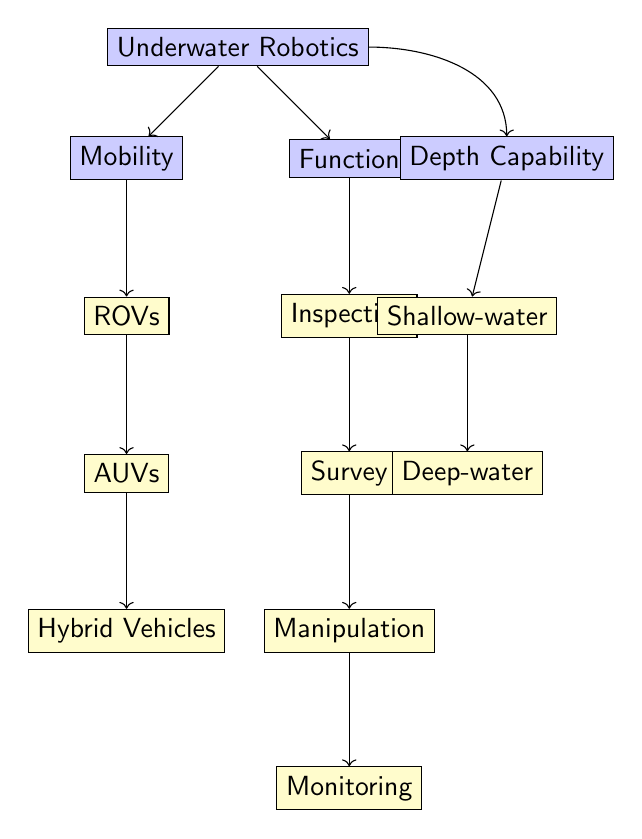
\begin{tikzpicture}[
	node distance=2cm and 2cm,
	every node/.style={draw, align=center, font=\sffamily},
	bluebox/.style={fill=blue!20},
	yellowbox/.style={fill=yellow!20}
	]
	
	% Nodes
	\node[bluebox] (root) {Underwater Robotics};
	\node[bluebox, below left of=root] (mobility) {Mobility};
	\node[bluebox, below right of=root] (function) {Function};
	\node[bluebox, right of=function] (depth) {Depth Capability};
	
	\node[yellowbox, below of=mobility] (rcvs) {ROVs};
	\node[yellowbox, below of=rcvs] (auvs) {AUVs};
	\node[yellowbox, below of=auvs] (hybrid) {Hybrid Vehicles};
	
	\node[yellowbox, below of=function] (inspection) {Inspection};
	\node[yellowbox, below of=inspection] (survey) {Survey};
	\node[yellowbox, below of=survey] (manipulation) {Manipulation};
	\node[yellowbox, below of=manipulation] (monitoring) {Monitoring};
	
	\node[yellowbox, below of=depth, xshift=-0.5cm] (shallow) {Shallow-water};
	\node[yellowbox, below of=shallow] (deep) {Deep-water};
	
	% Arrows with custom angles
	\draw[->] (root) -- (mobility);
	\draw[->] (root) -- (function);
	\draw[->] (root) to[out=0, in=90] (depth); % Adjusted angle to avoid crossing
	
	\draw[->] (mobility) -- (rcvs);
	\draw[->] (rcvs) -- (auvs);
	\draw[->] (auvs) -- (hybrid);
	
	\draw[->] (function) -- (inspection);
	\draw[->] (inspection) -- (survey);
	\draw[->] (survey) -- (manipulation);
	\draw[->] (manipulation) -- (monitoring);
	
	\draw[->] (depth) -- (shallow);
	\draw[->] (shallow) -- (deep);
	
\end{tikzpicture}
	
\section{Methodology}
\lipsum[2]  % Remove this and write your own methodology
	
\section{Results and Discussion}
\lipsum[3]  % Remove this and write your results and discussion
	
\section{Conclusion}
\lipsum[4]  % Remove this and write your conclusion
	
\section*{Acknowledgments}
Here you can acknowledge people who contributed but are not listed as co-authors.


\printbibliography

	
\end{document}
